\section{Основные определения}

species
HSet
h-species
аналитический функтор

\section{Формулы}

\subsection{Аналитический функтор для h-species}
Аналитический функтор $\mathcal F$ соответствующий species $F$ является
продуктивной конструкцией, позволяющей определить композиционное произведение
species. Вводить его можно разными способами, мы ограничимся универсальным
свойством и явной конструкцией (TODO: дописать и возможно добавить определение
Дурова). Аналитический функтор является левым расширением по Кану функтора $F$
относительно $i$.

\begin{tikzpicture}
\label{comm:an}
	\node (B) {$B$};
	\node (S1) [below of=B] {$Set$};
	\node (S2) [right of=B, node distance=3cm] {$Set$};
	\draw [right hook->] (B) to node [swap] {$i$} (S1);
	\draw [->] (B) to node {$F$} (S2);
	\draw [->] (S1) to node [swap] {$\mathcal F$} (S2);	
\end{tikzpicture}

Эта диаграмма не является коммутативной, а коммутативна лишь настолько, насколько может быть коммутативной диаграмма
подобного вида. А именно, имеется  естественное преобразование  $\kappa F\rightarrow i \circ \mathcal F$,
обладающее следующим универсальным свойством:
 для любого функтора $M \colon
Set \rightarrow Set$ и морфизма функторов $\eta \colon F \rightarrow i \circ M$
этот морфизм пропускаеться через $\mathcal F$ при помощи $\kappa$.

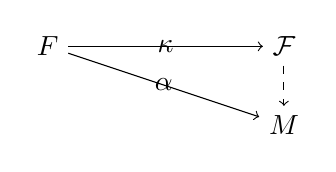
\begin{tikzpicture}
\label{comm:an-uni}
	\node (F) {$F$};
	\node (Fm) [right of=F, node distance=3cm] {$\mathcal F$};
	\node (M) [below of=Fm] {$M$};
	\draw [->] (F) to node {$\kappa$} (Fm);
	\draw [->] (F) to node [swap] {$\alpha$} (M);
	\draw [->, dashed] (Fm) to node [swap] {} (M);
\end{tikzpicture}


Явная формула для аналитического функтора. Для доказательства см (TODO)
\begin{equation}
\label{eq:an}
	\mathcal F = \sum\limits_n F[n] \times A^n / S_n
\end{equation}

У аналитического функтора для типа структуры $F$ имеется прозрачный комбинаторная интерпретация.
Если трактовать множество $A$ как набор цветов,
то значение аналитического функтора $\mathcal F(A)$ трактуется как множество структур типа $F$
раскрашенных в цвета из $A$.

Хочется построить аналог аналитического функтора для h-species

\begin{tikzpicture}
\label{comm:h-an}
	\node (B) {$HB$};
	\node (S1) [below of=B] {$HSet$};
	\node (S2) [right of=B, node distance=3cm] {$HSet$};
	\draw [right hook->] (B) to node [swap] {$i$} (S1);
	\draw [->] (B) to node {$F$} (S2);
	\draw [->] (S1) to node [swap] {$\mathcal F$} (S2);
\end{tikzpicture}

\begin{equation}
\label{eq:h-an}
	\mathcal F = \sum\limits_n F[\Bar n] \times A^{\Bar n} / B_n
\end{equation}
Где $A^{\Bar n}$ задает отображение, сохраняющее инволюцию. 

TODO:Здесь нужно добавить проверук универсальности картинки

\subsection{Декатегорификация аналитического функтора: Фробениусова
характеристика / Цикленный индекс} 
\subsubsection{Случай обычных species}
Напомним ситуацию с обычными species.
Процедура декатегорификации не имеет строго математического смысла, так же как и процедура квантования.
Сейчас мы предложим процедуру, которая, стартуя с обычных species,
на выходе дает классический цикленный инлдекс/фробениусову характеристику.
Затем мы попытаемся аналогические действия провести и в гипероктаэдральном случае.
Декатегорификацией моноидальной категории $\mathbb B$ является моноид классов изоморфизма объектов категории
$\mathbb B$, то есть моноид натуральных чисел по сложению.
Декатегорификкацией $\widehat{\mathbb B}$ естественным образом оказывается
моноидная алгебра с коэффициентами из $\mathbb Z$ для моноида $\mathbb N$, то есть кольцо многочленов $Z[X]$.
(Правда это не то, что мы хотели. Чтобы получить цикленный индекс надо декатегорифицировать
саму операцию подстановки и аналитический функтор).

Надо устроить морфизм из моноидальной
категории (категории с тензорным произведением) в какую-нибудь алгебру функций. Мы вводим весовую
функцию таким образом что орбита раскрашенной структуры под действием $S_n$ имеет один и тот же вес.
После этого можно задать вопрос о коэфициенте при мономе, отвечающем весу. Это
будет число орбит с заданной весовой функцией. По Лемме Бернсайда это то же
самое, что и усредненное число неподвижных точек по всем элементам группы. Чтобы
раскрашенная структура была неподвижна под действием перестановки $\sigma$
нужно, чтобы во-первых она была неподвижна как не раскрашенная структура, а
во-вторых расскраска должна переходить в себя. В качестве
весовой функции выбираем моном возникающий в произведении переменных отвечающим
цветам. Например расскраске в которой 2 первых цвета и 1 второй
соответсвует моном $x_1^2x_2$. Тогда первое условие дает нам сомножитель
$\chi(\sigma)$, где характер это характер соответствующего перестановочного
представления с базисом из структур. Второе условие требует покраски каждого
цикла в один и тот же цвет. Итоговая формула называеться фробениусовой
характеристикой / цикленным индексом. Она считает количество неподвижных
раскрашенных структур в среднем. 

\begin{equation}
\label{eq:fr}
\mathcal Z_F =
\sum_{n}\frac{1}{n!}\sum_{\sigma \in S_n}\chi(\sigma)\psi^{\lambda(\sigma)} =
\sum_{n, \lambda \vdash n}\chi(\sigma_{\lambda})
\frac{\psi^{\lambda}}{z_{\lambda}}
\end{equation}

Где $\chi$ --- характер (перестановочного) представления заданного $F$, $\sigma$
--- перестановка цикленного типа $\lambda$, 
$\psi^{\lambda} = 
(x_1^{\lambda_1} + x_2^{\lambda_1} + x_3^{\lambda_1} + \dots)
(x_1^{\lambda_2} + x_2^{\lambda_2} + x_3^{\lambda_2} + \dots)
(x_1^{\lambda_3} + x_2^{\lambda_3} + x_3^{\lambda_3} + \dots)
\dots$,
 $z_\lambda$ --- индекс класса сопряженности $\sigma$.
Появляется она из следующих соображений: в числителе стоит симметрическая
функция считающая все неподвижные раскраски. Цвета это $x_1, x_2, x_3, \dots$

\subsubsection{Случай h-species}
Попробуем построить аналогичную конструкцию для h-species.
Прежде всего отметим, что раскраска, элемент $A^{\Bar n}$, это отображение,
сохраняющее инволюцию. Значит элементы $n$ и $-n$ должны отображаться либо в
один и тот же элемент $A$ (который инволюцией переводиться в себя), либо в пару
элементов сопряженных инволюцией. Будем называть первый случай
\emph{моноцветом}, второй --- \emph{бицветом}.	

Покрашенные структуры сами по себе можно рассматривать как моноцвет, либо
бицвет. Это по--прежнему определяется длинной орбиты инволюции $A$, уже
после факторизации по $B_n$. То есть кроме действия $B_n$ есть еще внешняя
инволюция --- действие $Z_2$. Будем называть их \emph{моноструктурами} и
\emph{биструктурами}.

Цикленный индекс, считающий только моноструктуры будем обозначать
$\mathcal Z^{(1)}$, биструктуры --- $\mathcal Z^{(2)}$. Количество орбит под
действием $H_n \times Z_2$ соответствует $\mathcal Z^{(1)} + \mathcal Z^{(2)}$,
а под действием только $H_n$ соответствует $\mathcal Z^{(1)} + 2\mathcal
Z^{(2)}$. Поскольку каждая биструктура будет посчитан два раза.

В качестве H-множества цветов возьмем счетное множество моноцветов $x_1, x_2,
x_3, \dots$ объединенное с счетным множеством бицветов $y_1, y_2, y_3, \dots$.

Допустим, что мы придумали весовую функцию, отправляющую каждую расскрашенную
структуру в моном и любая орбита отправляеться в один моном. Применив Лемму
Бернсайда переходим к подсчету неподвижных точек. Циклы в каждом элементе $H_n$
бывают двух типов:
длинные --- каждая грань входит в цикл вместе со своей противоположной гранью и
короткие --- пара граней лежит в симметричных, различных циклах. 

Посчитаем количество количество неподвижных точек для $H_n$. Пусть $\lambda^1$
--- цикленный тип коротких перестановок, $\lambda^2$ --- цикленный тип длинных
перестановок. Утверждение: неподвижные раскрашенные структуры, это в точности
те, у которых длинный цикл соответсвует моноцвету, а пара симметричных коротких 
может быть покрашена либо в моноцвет, либо в бицвет.

Это можно выразить такой формулой:
\begin{equation}
\label{eq:h-fr1}
\begin{split}
\mathcal Z_F^{(1)} + 2\mathcal Z_F^{(2)} = 
\sum_{n}\frac{1}{2^{n}n!}\sum_{\sigma \in B_n}&\chi(\sigma)
\psi_{x, y, y}^{\lambda^1(\sigma)} \psi_{x}^{\lambda^2(\sigma)} = \\
\sum_{n, \lambda^1 + \lambda^2 \vdash n}&\chi(\sigma_{\lambda^1 \lambda^2})
\frac{\psi_{x, y, y}^{\lambda^1} \psi_{x}^{\lambda^2}}{z_{\lambda^1 \lambda^2}}
\end{split}
\end{equation}
Здесь нижний индекс $\psi$ означает переменные по которым берется степенная
сумма. Например $\psi_{x, y, y}^2 =  (x_1^2 + x_2^2 + x_3^2 + \dots + y_1^2 +
y_2^2 + y_3^2 + \dots + y_1^2 + y_2^2 + y_3^2 + \dots)$. При этом коофициент
2 у $y_i^2$ отражает тот факт, что можно раскрасить $k$ пар граней в бицвет,
так чтобы расскраска была неподвижна, под действием короткого цикла, 2-мя способами.

Посчитаем количество количество неподвижных точек для $H_n \times Z_2$. Разобъем
сумму на две части --- $(h, \Bar 0)$ и $(h, \Bar 1)$. Для первой формула будет
аналогична \ref{eq:h-fr1}, только из-за того что порядок группы в 2 раза больше,
появится коофициент $\frac{1}{2}$.

Во второй части по-прежнему можно красить и длинные и короткие циклы в моноцвет.
А вот с бицветом происходит любопытная вещь --- предположим мы красим цикл (пару
циклов в него). Тогда добавляется смена грани на каждом шаге, а значит для
циклов нечетной длинны сменится свойство короткий--длинный. Итоговая формула
такая 

\begin{equation}
\begin{split}
\mathcal Z_F^{(1)} + \mathcal Z_F^{(2)} = 
\frac{1}{2}&
\sum_{n, \lambda^1 + \lambda^2 \vdash n}\chi(\sigma_{\lambda^1 \lambda^2})
\frac{\psi_{x, y, y}^{\lambda^1} \psi_{x}^{\lambda^2}}{z_{\lambda^1 \lambda^2}}
+ \\
\frac{1}{2}&
\sum_{n, \lambda_o^1 + \lambda_o^2 + \lambda_e^1 + \lambda_e^2 \vdash
n}\chi(\sigma_{\lambda_o^1 \lambda_o^2 \lambda_e^1 \lambda_e^2})
\frac{\psi_{x, y, y}^{\lambda_e^1 + \lambda_o^2} \psi_{x}^{\lambda_e^2 + 
\lambda_o^1}}{z_{\lambda_o^1 \lambda_o^2 \lambda_e^1 \lambda_e^2}}
\end{split}
\end{equation}

Где $\lambda_o$ --- циклы нечетной длинны, $\lambda_e$ ---
циклы четной длинны.

Откуда легко получить
\begin{equation}
\label{eq:h-fr2}
\mathcal Z_F^{(1)} = 
\sum_{n, \lambda_o^1 + \lambda_o^2 + \lambda_e^1 + \lambda_e^2 \vdash
n}\chi(\sigma_{\lambda_o^1 \lambda_o^2 \lambda_e^1 \lambda_e^2})
\frac{\psi_{x, y, y}^{\lambda_e^1 + \lambda_o^2} \psi_{x}^{\lambda_e^2 + 
\lambda_o^1}}{z_{\lambda_o^1 \lambda_o^2 \lambda_e^1 \lambda_e^2}}
\end{equation}

\begin{equation}
\begin{split}
\mathcal Z_F^{(2)} = 
\frac{1}{2}&
\sum_{n, \lambda^1 + \lambda^2 \vdash n}\chi(\sigma_{\lambda^1 \lambda^2})
\frac{\psi_{x, y, y}^{\lambda^1} \psi_{x}^{\lambda^2}}{z_{\lambda^1 \lambda^2}}
- \\
\frac{1}{2}&
\sum_{n, \lambda_o^1 + \lambda_o^2 + \lambda_e^1 + \lambda_e^2 \vdash
n}\chi(\sigma_{\lambda_o^1 \lambda_o^2 \lambda_e^1 \lambda_e^2})
\frac{\psi_{x, y, y}^{\lambda_e^1 + \lambda_o^2} \psi_{x}^{\lambda_e^2 + 
\lambda_o^1}}{z_{\lambda_o^1 \lambda_o^2 \lambda_e^1 \lambda_e^2}}
\end{split}
\end{equation}

\subsubsection{Примеры}
Посчитаем цикленные индексы для простых h-species.
Здесь мы будем писать $Z(A)$ вместо $Z_A$. Это не должно вызывать путаницу,
поскольку вместо $A$ будут использоваться схематические картинки и их
не перепутать с переменными, от которых считаеться цикленный индекс. 

Структура <<одна пара граней>>, будем символически писать \dA.
$$
\Zfull(\dA) = \frac{1}{2}(\psi_{x,y,y}^1 + \psi_{x}^1) = \psi_{x,y}^1
$$
$$
\mathcal Z^{(1)}(\dA) = \frac{1}{2}(\psi_{x}^1 + \psi_{x, y, y}^1) = \psi_{x,y}^1
$$
Значит
$$
\mathcal Z^{(2)}(\dA) = 0
$$

Структура <<одна пара граней, грани различаются>>. Обозначение \dB.
$$
\Zfull(\dB) = \frac{1}{2}(2\psi_{x,y,y}^1 + 0\psi_{x}^1) = \psi_{x,y,y}^1
$$
$$
\mathcal Z^{(1)}(\dB) = \frac{1}{2}(2\psi_{x}^1 + 0\psi_{x, y, y}^1) = \psi_{x}^1
$$
Значит
$$
\mathcal Z^{(2)}(\dA) = \psi_{y}^1
$$

Структура <<квадрат>>. Обозначение \dAA.
$$
\Zfull(\dAA) = \frac{1}{8}((\psi_{x,y,y}^1)^2 + (\psi_{x}^1)^2 + 2\psi_{x}^2 +
2(\psi_x^1\psi_{x,y,y}^1) + 2\psi_{x,y,y}^2)
$$
Здесь коофициенты --- не характеры (характер при каждом слагаемом $= 1$).
$$
\mathcal Z^{(1)}(\dAA) = \frac{1}{8}((\psi_{x}^1)^2 + (\psi_{x, y, y}^1)^2 +
2\psi_{x, y, y}^2 + 2(\psi_{x, y, y}^1\psi_{x}^1) + 2\psi_{x}^2) = \Zfull(\dAA)
$$
Последнее следовало и из общих соображений: легко видеть что $\mathcal
Z^{(2)}(\dAA) = 0$.

Структура <<квадрат, противоположные грани различаются>>. Обозначение \dBB.
$$
\Zfull(\dBB) = \frac{1}{8}(4(\psi_{x,y,y}^1)^2 + 0(\psi_{x}^1)^2 + 0\psi_{x}^2
+ 0(\psi_x^1\psi_{x,y,y}^1) + 2\times2\psi_{x,y,y}^2)
$$
$$
\mathcal Z^{(1)}(\dBB) = \frac{1}{8}(4(\psi_{x}^1)^2 + 2\times2\psi_{x,y,y}^2)
$$
Откуда
$$
\mathcal Z^{(2)}(\dBB) = \frac{1}{2}(\Zfull(\dBB) - \mathcal
Z^{(1)}(\dBB)) = \frac{1}{2}(\psi_{y,y}^1\psi_{x}^1 +
\frac{1}{2}(\psi_{y, y}^1)^2) = \psi_{y}^1\psi_{x}^1 + (\psi_{y}^1)^2 $$

Структура $\dB \times \dB$. Это не то же самое что \dBB, поскольку это <<упорядоченная пара \dB>>.
Ее цикленный индекс мы посчитаем дальше.

\subsection{Сумма и произведение цикленных индексов}
\subsubsection{Сумма}
Сумма цикленных индексов соответсвует поточечной сумме аналитических
функторов и здесь нет никаких сюрпризов:
$$
\mathcal Z_{A + B}^{(1)} = \mathcal Z_A^{(1)} + \mathcal Z_B^{(1)}
$$
$$
\mathcal Z_{A + B}^{(2)} = \mathcal Z_A^{(2)} + \mathcal Z_B^{(2)}
$$
\subsection{Произведение}
Для произведения уже не совсем так. Утверждается, что моноструктура получается
в произведении двух моноструктур. А биструктура получается, если один из
сомножителей биструктура. Причем в случае, когда оба сомножителя ---
биструктуры, получается две различных биструктуры. То есть
$$
\mathcal Z_{A * B}^{(1)} = \mathcal Z_A^{(1)} * \mathcal Z_B^{(1)}
$$
$$
\mathcal Z_{A * B}^{(2)} = 
\mathcal Z_A^{(1)} * \mathcal Z_B^{(2)} + 
\mathcal Z_A^{(2)} * \mathcal Z_B^{(1)} +
2 (\mathcal Z_A^{(2)} * \mathcal Z_B^{(2)})
$$
Откуда следует
$$
(\mathcal Z_{A * B}^{(1)} + 2\mathcal Z_{A * B}^{(2)}) = 
(\mathcal Z_A^{(1)} + 2\mathcal Z_A^{(2)}) * 
(\mathcal Z_B^{(1)} + 2\mathcal Z_B^{(2)})
 $$
Что логично, поскольку $(\mathcal Z_F^{(1)} + 2\mathcal Z_F^{(2)})$ --- это
цикленный индекс для цветов, с <<забытой>> инволюцией.

\subsubsection{Примеры}
Посчитаем произведение уже известных h-структур и их цикленных индексов.

Структура $\dA \times \dA$.
$$
\mathcal Z^{(1)}(\dA \times \dA) = \mathcal Z^{(1)}(\dA) \times \mathcal
Z^{(1)}(\dA) = (\psi_{x, y}^1)^2
$$

Структура $\dB \times \dB$.
$$
\Zfull(\dB \times \dB) = \Zfull(\dB) \times \Zfull(\dB) =(\psi_{x, y, y}^1)^2
$$
Легко получить эту же формулу и из других соображений, как
$\frac{1}{8}(8(\psi_{x, y, y}^1)^2)$.
$$
\mathcal Z^{(1)}(\dB \times \dB) = \mathcal Z^{(1)}(\dB) \times \mathcal
Z^{(1)}(\dB) =(\psi_{x}^1)^2
$$

\subsection{Цикленный индекс композиции}
\subsubsection{Случай обычных species}
Аналитический функтор позволяет дать определние композиционного произведения
двух структур. Рассмотрим два species $F$ и $G$. По ним можно построить
аналитические функторы $\mathcal F$ и $\mathcal G$. Композиция этих функторов
снова будет анлитическим функтором $\mathcal F \circ \mathcal G$. Доказательство
его аналитичности можно найти в [TODO: где или взять доказательство Дурова].
Species который соответсвует цикленному индексу $\mathcal F \circ \mathcal G$ и
будет называться $F \circ G$. У этого определения есть простая, наглядная
комбинаторная интерпретация: каждую точку структуры $F$ раздуваем(красим) в
структуру типа $G$. Чудесный факт заключается в том, что в декатегорификации
композиция соответствует простой формуле подстановки. Сейчас мы ее напишем и
приведем набросок доказательства. В качестве множества цветов $A$ рассмотрим
счетный набор цветов $x_1, x_2, x_3, \dots$ Цикленный индекс запишем
относительно базиса кольца симметрических функций $\psi^1, \psi^2, \psi^3, \dots$
\begin{multline}
\label{eq:zfg}
	\mathcal Z_{F \circ G} (\psi^1, \psi^2, \psi^3, \dots) = \\
	\mathcal Z_F(
		\mathcal Z_G(\psi^1, \psi^2, \psi^3, \dots),
		\mathcal Z_G(\psi^2, \psi^4, \psi^6, \dots),
		\mathcal Z_G(\psi^3, \psi^6, \psi^9, \dots),
		\dots
	)
\end{multline}

В композиции двух аналитических функторов получается, что цвета в которые мы
красим структуру $F$ это структуры типа $G$. То есть $\mathcal Z_{F \circ G} =
\mathcal Z_F(\psi_g^1, \psi_g^2, \psi_g^3, \dots)$, где $\psi_g^i = (g_1^i +
g_2^i + g_3^i + \dots)$, где $g_i$ --- перечисление всех структур типа $G$.
Нужно раскрыть переменные $g_i $ --- написать их относительно начальных цветов.
Формулу $\psi_g^i = \mathcal Z_G(\psi^i, \psi^{2i}, \psi^{3i}, \dots)$ легко
понять в переменных $x_1, x_2, x_3, \dots$. Мы должны покрасить $i$ кусков в
одну и ту же $G$--структуру. Значит каждый цвет $x_j$ заменяется на $x_j^i$.

Формулу \ref{eq:zfg} можно специализировать для подсчета labeled--структур. То
есть покрашенных структур у которых нет двух одинаковых цветов в расскраске.
Соответсвующие мономы (в базисе $x_1, x_2, x_3, \dots$) возникают только при
раскрытии мономов вида $c(\psi^1)^k$ и коэффициент в них равен $ck!$ --- такой
же как при мономе с точностью до факториала. Этот факториал приводит к
необходимости рассматривать экспоненциальные производящие функции вместо
обычных. Можно занулить все остальные мономы подстановкой $\psi^1 = t, \psi^2 =
0, \psi^3 = 0, \psi^4 = 0$. Формула \ref{eq:zfg} примет вид $
\mathcal Z_{F \circ G} (t, 0, 0, \dots) =
	\mathcal Z_F(
		\mathcal Z_G(t, 0, 0, \dots), 0, 0, \dots
	)
$.
А значит для экспоненциальных производящих функции labeled-структур справедливо
равенство
\begin{equation}
\label{eq:comp}
(f \circ g) (t) = f(g(t))
\end{equation}
А поскольку labeled структур ровно в $k!$ раз больше, чем unlabeled, то
равенство \ref{eq:comp} справедливо для обыкновенных производящих функций
unlabeled структур.

\subsubsection{Случай h-species}
Теперь попробуем выстроить теорию композиции цикленного индекса для h-species,
параллельно теории species. Прежде всего отметим, что инволюция на множестве
цветов делит их на моноцвета ($x_1, x_2, x_3, \dots$) и бицвета ($y_1, y_2,
y_3, \dots$). Однако, формулы \ref{eq:h-fr1} и \ref{eq:h-fr2} подсказывают, что
в качестве базиса можно брать не $\psi_x^i, \psi_y^j$ а $\psi_x^i, \psi_{x,y,y}^j$. Впрочем это
тривиальная замена переменных.

Итак мы хотим выяснить чему равняются
\begin{equation*}
\begin{split}
\mathcal Z^{(1)}_{F \circ G} (&\psi_x^1, \psi_x^2, \psi_x^3, \dots, \\
						&\psi_{x,y,y}^1, \psi_{x,y,y}^2, \psi_{x,y,y}^3, \dots)
\end{split}
\end{equation*}

\begin{equation*}
\begin{split}
\mathcal Z^{(2)}_{F \circ G} (&\psi_x^1, \psi_x^2, \psi_x^3, \dots, \\
						&\psi_{x,y,y}^1, \psi_{x,y,y}^2, \psi_{x,y,y}^3, \dots)
\end{split}
\end{equation*}

Утверждается следующее:
\begin{equation}
\begin{split}
\label{eq:h-zfg}
	\mathcal Z^{(1)/(2)}_{F \circ G} (\psi_x^1, \psi_x^2, \psi_x^3, &\dots, 
	\psi_{x,y,y}^1, \psi_{x,y,y}^2, \psi_{x,y,y}^3, \dots) = \\
	\mathcal Z_F^{(1)/(2)}(
		&\mathcal Z^{(1)}_G(\psi_x^1, \psi_x^2, \psi_x^3, \dots, 
					 \psi_{x, y, y}^1, \psi_{x, y, y}^2, \psi_{x, y, y}^3, \dots), \\
		&\mathcal Z^{(1)}_G(\psi_x^2, \psi_x^4, \psi_x^6, \dots, 
					 \psi_{x, y, y}^2, \psi_{x, y, y}^4, \psi_{x, y, y}^6, \dots), \\
		&\mathcal Z^{(1)}_G(\psi_x^3, \psi_x^6, \psi_x^9, \dots, 
					 \psi_{x, y, y}^3, \psi_{x, y, y}^6, \psi_{x, y, y}^9, \dots), \\
		&\dots, \\
		&\Zfull_G(\psi_x^1, \psi_x^2, \psi_x^3, \dots, 
					 \psi_{x,y,y}^1, \psi_{x,y,y}^2, \psi_{x,y,y}^3, \dots), \\
		&\Zfull_G(\psi_x^2, \psi_x^4, \psi_x^6, \dots, 
					 \psi_{x,y,y}^2, \psi_{x,y,y}^4, \psi_{x,y,y}^6, \dots), \\
		&\Zfull_G(\psi_x^3, \psi_x^6, \psi_x^9, \dots, 
					 \psi_{x,y,y}^3, \psi_{x,y,y}^6, \psi_{x,y,y}^9, \dots), \\
		&\dots
	)
\end{split}	
\end{equation}
Эта формула слишком грамоздкая, поэтому давайте напишем ее на уровне членов:
\begin{equation*}
\begin{split}
\psi_x^i \circ (\mathcal Z^{(1)}_G, \mathcal Z^{(2)}_G ) = \mathcal Z^{(1)}_G
(&\psi_x^i, \psi_x^{2i}, \psi_x^{3i}, \dots, \\
&\psi_x^i, \psi_x^{2i}, \psi_x^{3i}, \dots)
\end{split}
\end{equation*}

\begin{equation*}
\begin{split}
\psi_{x,y,y}^i \circ (\mathcal Z^{(1)}_G, \mathcal Z^{(2)}_G ) = \Zfull_G
(&\psi_x^i, \psi_x^{2i}, \psi_x^{3i}, \dots, \\
&\psi_x^i, \psi_x^{2i}, \psi_x^{3i}, \dots)
\end{split}
\end{equation*}
Здесь мы пишем $(\mathcal Z^{(1)}_G, \mathcal Z^{(2)}_G )$, поскольку
цикленный индекс для h-species в действительности представляет собой пару.
Биструктуры подставляются вместо бицветов, моноструктуры, вместо моноцветов. В
остальном рассуждение дословно повторяет случай обычных species.

Аналогично, если сделать подстановку 
$$
\psi_{x}^1 = t, \psi_{x}^k = 0, k>1
$$
$$
\psi_{x,y,y}^1 = s, \psi_{x,y,y}^k = 0, k>1
$$

То полученная формула показывает, что \ref{eq:comp} справедливо для
экспоненциальных производящих функций bilabeled-структур (то есть производящая
функция от двух переменных). А можно сделать подстановку $s := t$, которая
даст выполнение формулы \ref{eq:comp} для exp-производящей функции просто
labeled-структур. А значит и обычной производящей функции unlabeled-структур.

\subsubsection{Примеры}
Посчитаем $(\mathcal Z^{(1)}, \mathcal Z^{(2)})(\dB \circ \dA)$
$$
\mathcal Z^{(1)}(\dB \circ \dA) = \psi_{x}^1 \circ \psi_{x, y}^1 = \psi_{x, y}^1
= \mathcal Z^{(1)}(\dA)
$$ 
$$
\mathcal Z^{(2)}(\dB \circ \dA) = \psi_{y}^1 \circ 0 = 0 = \mathcal Z^{(2)}(\dA)
$$
Да и вобще, справедливо
$$
\mathcal Z^{(1)}(\dB \circ A) = \mathcal Z^{(1)}(A)
$$ 
$$
\mathcal Z^{(2)}(\dB \circ A) = \mathcal Z^{(2)}(A)
$$
А так же
$$
\mathcal Z^{(1)}(A \circ \dB) = \mathcal Z^{(1)}(A)
$$ 
$$
\mathcal Z^{(2)}(A \circ \dB) = \mathcal Z^{(2)}(A)
$$
Это дает некоторое понимание композиции. Так $A \circ \dB = \dB \circ A = A$.
То есть \dB является нейтральным элементом в монойде h-species по композиции.
Это несколько контр-интуитивно, поскольку в обычных species нейтральным
элементом являеться одноточечное множество. А его образом при вложении species в
h-species являеться \dA. [TODO А не значит ли это что просто можно по другому вложить?]

Интересно посмотреть чем является \dA. Например
\begin{equation}
\begin{split}
\Zfull(\dBB \circ \dA) = \frac{1}{2} (\frac{1}{2}(\psi_{x,y,y}^1 +
\psi_{x}^1))^2 + \frac{1}{2} (\frac{1}{2}(\psi_{x,y,y}^2 +
\psi_{x}^2)) = \\
\frac{1}{8}((\psi_{x}^1)^2 + (\psi_{x, y, y}^1)^2 +
2\psi_{x, y, y}^2 + 2(\psi_{x, y, y}^1\psi_{x}^1) + 2\psi_{x}^2) =
\Zfull(\dAA)
\end{split}
\end{equation}
Откуда можно сделать вывод, что $\dBB \circ \dA = \dAA$.
То есть подстановка \dA, это <<стирание различий между противоположными
гранями>>.

\subsubsection{Предложения [TODO]}
$$(\mathcal Z^{(1)}_G, \mathcal Z^{(2)}_G)
(\psi_x^1, \psi_x^2, \psi_x^3, \dots, 
\psi_{x,y,y}^1, \psi_{x,y,y}^2, \psi_{x,y,y}^3, \dots)
 = (\mathcal Z_G(\psi_{x,y}^1, \psi_{x,y}^2, \psi_{x,y}^3, \dots), 0)$$
 Где $G$ --- обычный species, вложенный в h-species. А $\mathcal Z_G$ --- его
 цикленный индекс.
